% ===========================================================================
\section{Key Categories: Level Against Variance}
\label{sec:keycat}
% ===========================================================================

A key category is one with a significant influence on a national inventory's total. IPCC
Approach~1 sorts categories by their share of the absolute total and flags them cumulatively
to a \SI{95}{\percent} threshold. Thirteen of this inventory's \num{24} IPCC categories are key by that criterion.

We report a second ranking alongside it. A category's contribution to national variance is
$(E_x U_x)^2$ as a share of the sum over categories, from the same Approach-1 quadrature that
produces the national band. The level ranking says where emissions occur; the variance
ranking says where reduced uncertainty would most narrow the national interval.

\begin{table*}[htbp]
\centering
\footnotesize
\setlength{\tabcolsep}{5pt}
\begin{tabular}{@{}p{0.26\linewidth}llrrr@{}}
\toprule
\textbf{IPCC category} & \textbf{Code} & \textbf{Module} & \textbf{Mt} & \textbf{Level} &
\textbf{Var.} \\
 & & & \COe{} & (\%) & (\%) \\
\midrule
Enteric fermentation & 3.A.1 & agriculture & 151.66 & 34.1 & 63.05 \\
Road transportation & 1.A.3.b & transport & 40.19 & 9.0 & 0.95 \\
Public electricity and heat & 1.A.1.a & power & 40.04 & 9.0 & 0.80 \\
Manufacturing and construction & 1.A.2 & industry+power & 28.13 & 6.3 & 0.79 \\
Domestic wastewater & 4.D.1 & waste & 24.46 & 5.5 & 13.03 \\
Residential & 1.A.4.b & residential & 24.22 & 5.4 & 1.34 \\
Fugitive emissions, oil and gas$^{e}$ & 1.B.2 & fugitives & 23.50 & 5.3 & 3.33 \\
Cement production & 2.A.1 & ippu & 21.82 & 4.9 & 0.18 \\
Manure management & 3.A.2 & agriculture & 19.33 & 4.3 & 1.89 \\
Rice cultivation & 3.C.7 & agriculture & 16.55 & 3.7 & 4.31 \\
Direct N2O emissions from managed soils & 3.C.4 & agriculture & 16.43 & 3.7 & 3.95 \\
Indirect N2O emissions from managed soils & 3.C.5 & agriculture & 12.09 & 2.7 & 3.69 \\
Solid waste disposal & 4.A & waste & 9.17 & 2.1 & 2.27 \\
\midrule
\multicolumn{6}{@{}l}{\emph{Not key by level:}} \\
Urea application & 3.C.3 & agriculture & 4.82 & 1.1 & 0.01 \\
Open burning of waste & 4.C.2 & waste & 3.83 & 0.9 & 0.22 \\
Ammonia production & 2.B.1 & ippu & 3.24 & 0.7 & 0.00 \\
Indirect N2O emissions from manure management & 3.C.6 & agriculture & 1.90 & 0.4 & 0.18 \\
Agriculture/forestry/fishing$^{\dagger}$ & 1.A.4.c & transport & 1.73 & 0.4 & 0.01 \\
Biomass burning in croplands & 3.C.1.b & agriculture & 0.67 & 0.1 & 0.00 \\
Iron and steel production & 2.C.1 & ippu & 0.39 & 0.1 & 0.00 \\
Railways & 1.A.3.c & railways & 0.39 & 0.1 & 0.00 \\
Civil aviation & 1.A.3.a & aviation & 0.30 & 0.1 & 0.00 \\
Lubricant use & 2.D.1 & ippu & 0.08 & 0.0 & 0.00 \\
Railway stationary/off-road$^{\ddagger}$ & 1.A.2/1.A.4.c & railways & 0.005 & 0.0 & 0.00 \\
\bottomrule
\end{tabular}
\caption{The 1.A.1.a grid figure is the \texttt{power\_grid\_control} family reference; the family's other members read 38.45~Mt (fuel property), 44.05~Mt (coverage) and 57.82~Mt (legacy account), and none is a sensitivity.
$^{e}$~The 1.B.2 reference sits one membership step below the top of its own
9.601--24.694~Mt structural envelope, fertiliser feedstock being outside the post-meter
leakage base; the priced envelope members, including the 17.68~Mt geometric-mean
central reading, sit beside it in the configurations file.
National key-category analysis, IPCC Vol~1 Ch~4 Approach~1, screened over
\textbf{IPCC categories}. The first 11 cross the cumulative
\SI{95}{\percent} level threshold. \emph{A previous edition screened the engine's own
categories instead}, which split 1.A.2 between the power and industry modules and gave this
table \num{25} rows against the category table's \num{19}; the threshold, the ranking and
every variance share were computed on that second hierarchy. The engine categories are now
source streams beneath their code, in
\texttt{outputs/national\_key\_categories.csv}. $^{\dagger}$1.A.4.c's placement is unresolved:
the source's residual class mixes agricultural machinery with construction and industrial
plant that belongs under 1.A.2, and the split is not published. $^{\ddagger}$The rail
re-base's receiving category: the measured non-traction share of the railway fuel account
(workshops, power houses, pumps, track machinery), whose own 1.A.2-versus-1.A.4.c split the
Year Book does not publish. The variance column is a
different ranking, and it assumes categories are independent---see
Section~\ref{sec:uncertainty}. Level assessment only.}
\label{tab:keycat}
\end{table*}

\begin{figure}[htbp]
\centering
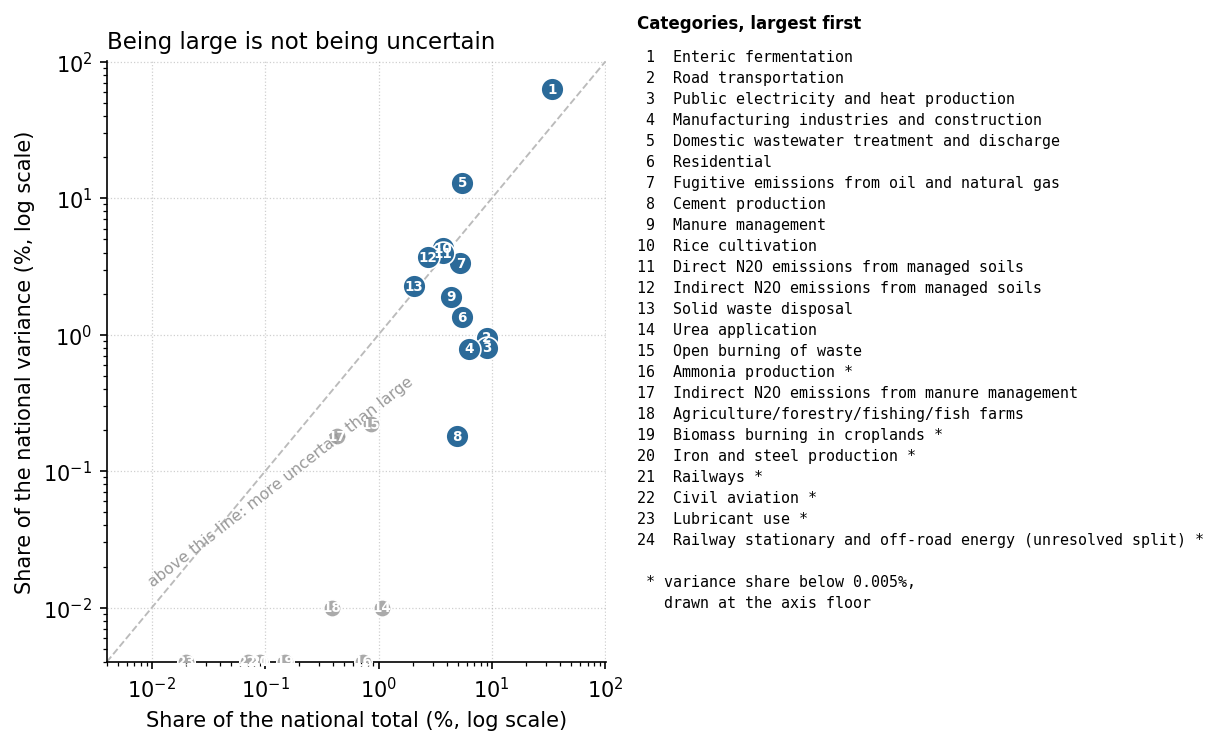
\includegraphics[width=\linewidth]{national_key_categories.png}
\caption{Level share against variance share for all \num{24} IPCC categories, on
\textbf{log axes}. The diagonal still marks equal level and variance share, so the reading is
unchanged: above it a category contributes more to national uncertainty than to magnitude. A
previous edition drew this linearly, which put enteric fermentation at one corner and
compressed eleven categories into a blot at the other---and the low corner is where the
finding is.}
\label{fig:keycat}
\end{figure}

\subsection{What the two rankings imply}

\textbf{Road transport} contributes \SI{9.0}{\percent} of emissions but
\SI{0.9}{\percent} of variance. Its fuel control and carbon factor constrain national mass,
so more fleet detail would improve composition and air-pollutant analysis more than the
national greenhouse-gas interval.

\textbf{Domestic wastewater} contributes \SI{5.5}{\percent} of emissions and
\SI{13.0}{\percent} of variance. It is the largest upward inversion after enteric
fermentation, and its uncertainty has two named drivers: the
methane correction factor for Pakistani sewers, now the larger term, and the
effluent N$_2$O factor's bounded 150-fold published range, which the 2019 Refinement
shortened from the 2006 Guidelines' 500-fold. Dissolved-methane sampling on urban drains
and an effluent-pathway N$_2$O measurement would test the two directly, in that order.

\textbf{Oil and gas fugitives} are now key by level. The completed 2019 segment account is
\SI{5.3}{\percent} of emissions and \SI{3.3}{\percent} of Approach-1 variance. This replaces
the earlier production-only result in which a very small category carried a four-order-of-
magnitude factor range. The remaining priority is no longer simply utility throughput: it is
technology and facility evidence for pipeline material, pressure, LDAR, compressors,
processing and wells.

\textbf{Enteric fermentation} remains dominant on both rankings, at
\SI{34.1}{\percent} of emissions and \SI{63.0}{\percent} of variance. The variance ranking
therefore supports work on both livestock and wastewater; it does not imply that one small
category alone controls national uncertainty.

\subsection{The ten-sector trend, and what its window can and cannot say}

IPCC's trend assessment requires a consistent series between one base and reference year.
All ten sectors now satisfy that requirement from FY2016--17 onward and are published as
the constant-scope view (Section~\ref{sec:series}), so the \emph{ten-sector} trend this
release previously declared out of reach is the one it supports. Cement and industrial
combustion were the two holding it back; both were absent for want of documents that turned
out to be held, and both now report every year of the window. The window now reaches
FY2015--16 as well: the product splits that blocked transport and industry there were
recovered from the publicly served Pakistan Oil Report 2015--2016 under a four-way identity
gate, so the full nine-year panel is a like-for-like base for the trend. The agriculture-only trend assessment carries a heavier qualification than
the others and it should be read with it: crop and nitrogen activity is now reconstructed on
Pakistani fiscal-year tables in every year, but enteric fermentation and manure management
still ride a calendar-year livestock projection because no fiscal enumeration of the herd
exists, so the sector's history is fiscal in the categories that could be moved and a
declared calendar projection in the \SI{77.37}{\percent} that could not
(Section~\ref{sec:agri-basis}).
